%implementing document formatting:
\documentclass[a4paper,11pt,fleqn,dvipsnames,oneside,openright,oldfontcommands]{memoir} 	% Openright aabner kapitler paa hoejresider (openany begge)


%%%%%%%%% Indsat random
%makes it possible to refer to the name of a chapter rather than just the number.
\usepackage{nameref}
\usepackage{pdfpages}
\usepackage{marvosym}
\usepackage{setspace}
\usepackage{graphicx} % For at sætte 2 billeder ved siden af hinanden

%package for writing program code in latex
\usepackage{listings}
%%%%%%%%%%%%%%%%%%%%%%

% ¤¤ Oversaettelse og tegnsaetning ¤¤ %
\usepackage[T1]{fontenc}					% Output-indkodning af tegnsaet (T1)
\usepackage[danish]{babel}					% Dokumentets sprog
\usepackage[utf8]{inputenc}					% Input-indkodning af tegnsaet (UTF8)
\usepackage{ragged2e,anyfontsize}			% Justering af elementer
\usepackage{fixltx2e}						% Retter forskellige fejl i LaTeX-kernen							
				
																							
% ¤¤ Figurer og tabeller (floats) ¤¤ %
\usepackage{graphicx} 						% Haandtering af eksterne billeder (JPG, PNG, EPS, PDF)
%\usepackage{eso-pic}						% Tilfoej billedekommandoer paa hver side
%\usepackage{wrapfig}						% Indsaettelse af figurer omsvoebt af tekst. \begin{wrapfigure}{Placering}{Stoerrelse}
\usepackage{multirow}                		% Fletning af raekker og kolonner (\multicolumn og \multirow)
\usepackage{multicol}         	        	% Muliggoer output i spalter
\usepackage{rotating}						% Rotation af tekst med \begin{sideways}...\end{sideways}
\usepackage{colortbl} 						% Farver i tabeller (fx \columncolor og \rowcolor)
\usepackage{xcolor}							% Definer farver med \definecolor. Se mere: http://en.wikibooks.org/wiki/LaTeX/Colors
\usepackage{flafter}						% Soerger for at floats ikke optraeder i teksten foer deres reference
\let\newfloat\relax 						% Justering mellem float-pakken og memoir
\usepackage{float}							% Muliggoer eksakt placering af floats, f.eks. \begin{figure}[H]
\usepackage{array,booktabs,xcolor,longtable} % kan lave \hdashline i tabellertabe
\usepackage{arydshln}
\usepackage{tabu}

	
	
% ¤¤ Matematik mm. ¤¤
\usepackage{amsmath , amsthm , amsfonts , amssymb, float, stmaryrd} 		% Avancerede matematik-udvidelser
%\usepackage{mathtools}						% Andre matematik- og tegnudvidelser
\usepackage{textcomp}                 		% Symbol-udvidelser (f.eks. promille-tegn med \textperthousand )
\usepackage{rsphrase}						% Kemi-pakke til RS-saetninger, f.eks. \rsphrase{R1}
\usepackage[version=3]{mhchem} 				% Kemi-pakke til flot og let notation af formler, f.eks. \ce{Fe2O3}
\usepackage{siunitx}						% Flot og konsistent praesentation af tal og enheder med \si{enhed} og \SI{tal}{enhed}
\sisetup{output-decimal-marker = {,}}		% Opsaetning af \SI (DE for komma som decimalseparator) 

% ¤¤ Referencer og kilder ¤¤ %
\usepackage[danish]{varioref}				% Muliggoer bl.a. krydshenvisninger med sidetal (\vref)
\usepackage[numbers]{natbib}				% Udvidelse med naturvidenskabelige citationsmodeller
%\usepackage{xr}							% Referencer til eksternt dokument med \externaldocument{<NAVN>}
%\usepackage{glossaries}					% Terminologi- eller symbolliste (se mere i Daleifs Latex-bog)
\usepackage{lastpage}					% Gør det mulig at refere til sidste side 

% ¤¤ Misc. ¤¤ %
\usepackage{listings}						% Placer kildekode i dokumentet med \begin{lstlisting}...\end{lstlisting}
\usepackage{lipsum}							% Dummy text \lipsum[..]
\usepackage[shortlabels]{enumitem}			% Muliggoer enkelt konfiguration af lister
\usepackage{pdfpages}						% Goer det muligt at inkludere pdf-dokumenter med kommandoen \includepdf[pages={x-y}]{fil.pdf}	
\pdfoptionpdfminorversion=6					% Muliggoer inkludering af pdf dokumenter, af version 1.6 og hoejere
\pretolerance=2500 							% Justering af afstand mellem ord (hoejt tal, mindre orddeling og mere luft mellem ord)


% Kommentarer og rettelser med \fxnote. Med 'final' i stedet for 'draft' udloeser hver note en error i den faerdige rapport.
\usepackage[footnote,draft,danish,silent,nomargin]{fixme}		


%%%% CUSTOM SETTINGS %%%%

% ¤¤ Marginer ¤¤ %
\setlrmarginsandblock{3.0cm}{2.5cm}{*}		% \setlrmarginsandblock{Indbinding}{Kant}{Ratio}
\setulmarginsandblock{2.5cm}{3.0cm}{*}		% \setulmarginsandblock{Top}{Bund}{Ratio}
\checkandfixthelayout 						% Oversaetter vaerdier til brug for andre pakker

%	¤¤ Afsnitsformatering ¤¤ %
\setlength{\parindent}{6mm}           		% Stoerrelse af indryk
\setlength{\parskip}{0mm}          			% Afstand mellem afsnit ved brug af double Enter
\linespread{1,1}							% Linie afstand



% ¤¤ Indholdsfortegnelse ¤¤ %
\setsecnumdepth{subsection}		 			% Dybden af nummerede overkrifter (part/chapter/section/subsection)
\maxsecnumdepth{subsection}					% Dokumentklassens graense for nummereringsdybde
\settocdepth{subsection} 					% Dybden af indholdsfortegnelsen

% ¤¤ Lister ¤¤ %
\setlist{
  topsep=0pt,								% Vertikal afstand mellem tekst og listen
  itemsep=-1ex,								% Vertikal afstand mellem items
} 

%hyperlinks in the tabel of contents - comment this out before the report is printed.
\usepackage{hyperref}
\hypersetup{
	bookmarks = true,  % Show 'bookmark'-frame in pdf.
	colorlinks = true, % True = colored links, False = framed links.
	citecolor = black,  % Link color for references.
	linkcolor = black,  % Link color in table of contents.
	urlcolor = black,   % Link color for extern URLs.
}

% ¤¤ Opsaetning af figur- og tabeltekst ¤¤ %
\usepackage{caption}
%\usepackage{subcaption}
\captionnamefont{\small\bfseries\itshape}	% Opsaetning af tekstdelen ('Figur' eller 'Tabel')
\captiontitlefont{\small}					% Opsaetning af nummerering
\captiondelim{. }							% Seperator mellem nummerering og figurtekst
\hangcaption								% Venstrejusterer flere-liniers figurtekst under hinanden
%\captionwidth{0.9\textwidth}					% Bredden af figurteksten
\setlength{\belowcaptionskip}{0pt}			% Afstand under figurteksten
\captionsetup[figure]{labelfont={bf,it},font={it}} % sætter nummer til fed og kursis. Resten til fed + skriften er mindre end resten
\captionsetup[table]{labelfont={bf,it},font={it}} 


% ¤¤ Opsaetning af listings ¤¤ %

\definecolor{commentGreen}{RGB}{34,139,24}
\definecolor{stringPurple}{RGB}{208,76,239}

\lstset{language=Matlab,					% Sprog
	basicstyle=\ttfamily\scriptsize,		% Opsaetning af teksten
	keywords={for,if,while,else,elseif,		% Noegleord at fremhaeve
			  end,break,return,case,
			  switch,function},
	keywordstyle=\color{blue},				% Opsaetning af noegleord
	commentstyle=\color{commentGreen},		% Opsaetning af kommentarer
	stringstyle=\color{stringPurple},		% Opsaetning af strenge
	showstringspaces=false,					% Mellemrum i strenge enten vist eller blanke
	numbers=left, numberstyle=\tiny,		% Linjenumre
	extendedchars=true, 					% Tillader specielle karakterer
	columns=flexible,						% Kolonnejustering
	breaklines, breakatwhitespace=true,		% Bryd lange linjer
}

% ¤¤ Navngivning ¤¤ %
\addto\captionsdanish{
	\renewcommand\appendixname{Bilag}
	\renewcommand\contentsname{Indholdsfortegnelse}	
	\renewcommand\appendixpagename{Bilag}
	\renewcommand\appendixtocname{Bilag}
	\renewcommand\cftchaptername{\chaptername~}				% Skriver "Kapitel" foran kapitlerne i indholdsfortegnelsen
	\renewcommand\cftappendixname{\appendixname~}			% Skriver "Appendiks" foran appendiks i indholdsfortegnelsen
}

% ¤¤ Kapiteludssende ¤¤ %
%\definecolor{numbercolor}{gray}{0.7}		% Definerer en farve til brug til kapiteludseende
%\newif\ifchapternonum

\makechapterstyle{AAU}
{
	% Afstand mellem sidehovedet og kapitel+tal+kapitelnavnet defineres til:
	\setlength{\beforechapskip}{0cm}

	% Afstanden mellem kapitelnavnet og body-teksten defineres til:
	\setlength{\afterchapskip}{2cm}

	% Typografiopsætningen til kapitel+tal defineres til:
	\renewcommand\chapnamefont{\sffamily\bfseries\LARGE\raggedright}
	
	% Typografiopsætningen til kapitel+tal defineres til:
	\renewcommand\chaptitlefont{\sffamily\bfseries\huge\color[cmyk]{1.00,0.38,0.00,0.64}}

	% Forårsager, at der til kapitlet også tilføjes dets respektive tal:
	\renewcommand\chapternamenum{}
	\renewcommand\printchapternum
	{
		\makebox[0pt][l]
		{
			\color[cmyk]{1.00,0.38,0.00,0.64}
			\hspace{0.1cm}
			\resizebox{!}{1cm}{\chapnamefont\bfseries\sffamily\thechapter}
		}
	}
	
	% Definitionen af linjenstykket mellem ``Kapitel #'' samt ``kapitelnavnet'':
			\renewcommand\afterchaptertitle{\par\hspace{1.5cm}\hrule height 1pt\vskip\midchapskip}
}

% Aktivering af selve kapitellayoutet med dét navn, som definerer kapitellayoutet (ses fra tidligere):
\chapterstyle{AAU}

%\makechapterstyle{jenor}{					% Definerer kapiteludseende frem til ...
%  \renewcommand\beforechapskip{0pt}
%  \renewcommand\printchaptername{}
%  \renewcommand\printchapternum{}
% % \renewcommand\printchapternonum{\chapternonumtrue}
%  \renewcommand\chaptitlefont{\fontfamily{pbk}\fontseries{db}\fontshape{n}\fontsize{20}{25}\selectfont\raggedright}
%  \renewcommand\chapnumfont{\fontfamily{pbk}\fontseries{m}\fontshape{n}\fontsize{1in}{0in}\selectfont\color{numbercolor}}
% \renewcommand\printchaptertitle[1]{
%    \noindent
%    \ifchapternum
%     \begin{tabularx}{\textwidth}{XI}
%	{\let\\\newline\chaptitlefont ##1\par}     
%    \end{tabularx}
%    \par\vskip-2.5mm\hrule
%    \else
%    \begin{tabularx}{\textwidth}{X}
%      {\parbox[b]{\linewidth}{\chaptitlefont ##1}} & \raisebox{-15pt}{\chapnumfont \thechapter}
%    \end{tabularx}
%    \par\vskip2mm\hrule
%    \fi
%  }
%}											% ... her
%
%\chapterstyle{jenor}						% Valg af kapiteludseende - Google 'memoir chapter styles' for alternativer

% ¤¤ Sidehoved ¤¤ %

\makepagestyle{AAU}							% Definerer sidehoved og sidefod udseende frem til ...
\makepsmarks{AAU}{%
	\createmark{chapter}{left}{shownumber}{}{. \ }
	\createmark{section}{right}{shownumber}{}{. \ }
	\createplainmark{toc}{both}{\contentsname}
	\createplainmark{lof}{both}{\listfigurename}
	\createplainmark{lot}{both}{\listtablename}
	\createplainmark{bib}{both}{\bibname}
	\createplainmark{index}{both}{\indexname}
	\createplainmark{glossary}{both}{\glossaryname}
}
\nouppercaseheads											% Ingen Caps oenskes

\makeoddhead{AAU}{Gruppe 17gr6403}{}{\leftmark}				% Definerer lige siders sidehoved (\makeevenhead{Navn}{Venstre}{Center}{Hoejre})
\makeevenhead{AAU}{\rightmark}{}{Aalborg Universitet}		% Definerer ulige siders sidehoved (\makeoddhead{Navn}{Venstre}{Center}{Hoejre})
\makeevenfoot{AAU}{Side \thepage\ af \pageref{LastPage}}{}{}							% Definerer lige siders sidefod (\makeevenfoot{Navn}{Venstre}{Center}{Hoejre})
\makeoddfoot{AAU}{}{}{Side \thepage\ af \pageref{LastPage}}								% Definerer ulige siders sidefod (\makeoddfoot{Navn}{Venstre}{Center}{Hoejre})
\makeheadrule{AAU}{\textwidth}{0.5pt}						% Tilfoejer en streg under sidehovedets indhold
\makefootrule{AAU}{\textwidth}{0.5pt}{1mm}					% Tilfoejer en streg under sidefodens indhold

\copypagestyle{AAUchap}{AAU}								% Sidehoved for kapitelsider defineres som standardsider, men med blank sidehoved
\makeoddhead{AAUchap}{}{}{}
\makeevenhead{AAUchap}{}{}{}
\makeheadrule{AAUchap}{\textwidth}{0pt}
\aliaspagestyle{chapter}{AAUchap}							% Den ny style vaelges til at gaelde for chapters
															% ... her
															
\pagestyle{AAU}												% Valg af sidehoved og sidefod


%%%% CUSTOM COMMANDS %%%%

% ¤¤ Billede hack ¤¤ %
\newcommand{\figur}[4]{
		\begin{figure}[H] \centering
			\includegraphics[width=#1\textwidth]{billeder/#2}
			\caption{#3}\label{#4}
		\end{figure} 
}

% ¤¤ Specielle tegn ¤¤ %
\newcommand{\decC}{^{\circ}\text{C}}
\newcommand{\dec}{^{\circ}}
\newcommand{\m}{\cdot}


%%%% ORDDELING %%%%

\hyphenation{}

%%%%Fra engelsk til dansk i \autoref{•} %%%%
\renewcommand{\figureautorefname}{figur}
\renewcommand{\sectionautorefname}{afsnit}
\renewcommand{\subsectionautorefname}{afsnit}
\renewcommand{\subsubsectionautorefname}{afsnit}
\renewcommand{\tableautorefname}{tabel}
\renewcommand{\appendixautorefname}{bilag}
\renewcommand{\equationautorefname}{ligning}
\renewcommand{\itemautorefname}{punkt}
\renewcommand{\chapterautorefname}{kapitel}
%Figure references:
\newcommand{\figref}[1]{\textbf{figur \ref{#1}}}

%Figure references after full stop/period:
\newcommand{\Figref}[1]{\textbf{Figur \ref{#1}}}

%Table references:
\newcommand{\tableref}[1]{\textbf{tabel \ref{#1}}}

%Table references after full stop/period:
\newcommand{\Tableref}[1]{\textbf{Tabel \ref{#1}}}

%Units:
%inserting '\omit' before '{\put' prior ot final compile will fix allignment (and generate errors)
\newcommand{\unit}[1]{{\put(300,0){$\hfill\left[\: #1 \:\right]$}}}

%Text:
\newcommand{\tx}[1]{\text{#1}}

%Equation references:
%1 equation:
\renewcommand{\eqref}[1]{\textbf{ligning (\ref{#1})}}
%2 equations:
\newcommand{\eqrefTwo}[2]{\textbf{ligning (\ref{#1})} and \textbf{(\ref{#2})}}
%3 equations:
\newcommand{\eqrefThree}[3]{\textbf{ligning (\ref{#1})}, \textbf{(\ref{#2})} and \textbf{(\ref{#3})}}
%4 equations:
\newcommand{\eqrefFour}[4]{\textbf{ligning (\ref{#1})}, \textbf{(\ref{#2})}, \textbf{(\ref{#3})} and \textbf{(\ref{#4})}}
%5 equations:
\newcommand{\eqrefFive}[5]{\textbf{ligning (\ref{#1})}, \textbf{(\ref{#2})}, \textbf{(\ref{#3})}, \textbf{(\ref{#4})} and \textbf{(\ref{#5})}}
%5 equations:
\newcommand{\eqrefSix}[6]{\textbf{ligning (\ref{#1})}, \textbf{(\ref{#2})}, \textbf{(\ref{#3})}, \textbf{(\ref{#4})}, \textbf{(\ref{#5})} and \textbf{(\ref{#6})}}
%5 equations:
\newcommand{\eqrefSeven}[7]{\textbf{ligning (\ref{#1})}, \textbf{(\ref{#2})}, \textbf{(\ref{#3})}, \textbf{(\ref{#4})}, \textbf{(\ref{#5})}, \textbf{(\ref{#6})} and \textbf{(\ref{#7})}}

%Equation references after full stop/period:
%1 equation:
\newcommand{\Eqref}[1]{\textbf{Ligning (\ref{#1})}}
%2 equations:
\newcommand{\EqrefTwo}[2]{\textbf{Ligning (\ref{#1})} and \textbf{(\ref{#2})}}
%3 equations:
\newcommand{\EqrefThree}[3]{\textbf{Ligning (\ref{#1})}, \textbf{(\ref{#2})} and \textbf{(\ref{#3})}}
%4 equations:
\newcommand{\EqrefFour}[4]{\textbf{Ligning (\ref{#1})}, \textbf{(\ref{#2})}, \textbf{(\ref{#3})} and \textbf{(\ref{#4})}}
%5 equations:
\newcommand{\EqrefFive}[5]{\textbf{Ligning (\ref{#1})}, \textbf{(\ref{#2})}, \textbf{(\ref{#3})}, \textbf{(\ref{#4})} and \textbf{(\ref{#5})}}
%5 equations:
\newcommand{\EqrefSix}[6]{\textbf{Ligning (\ref{#1})}, \textbf{(\ref{#2})}, \textbf{(\ref{#3})}, \textbf{(\ref{#4})}, \textbf{(\ref{#5})} and \textbf{(\ref{#6})}}
%5 equations:
\newcommand{\EqrefSeven}[7]{\textbf{Ligning (\ref{#1})}, \textbf{(\ref{#2})}, \textbf{(\ref{#3})}, \textbf{(\ref{#4})}, \textbf{(\ref{#5})}, \textbf{(\ref{#6})} and \textbf{(\ref{#7})}}
\raggedbottom % Soerger for at LaTeX ikke "straekker" teksten
\begin{document}


\frontmatter	 % Forindhold - nummereres med romertal

%implementing title sheet:
\clearpage
\thispagestyle{empty}

%\begin{figure}[H]
%	\raggedleft
%		
\includegraphics[width=0.2\textwidth]{figures/aaulogo-da.png}
%\end{figure}


%\vspace*{\fill} 
%\begin{center}	
%	\begin{Huge}
%		P3 Projektrapport - efterår 2015\\
%		\vspace{5 mm}
%		\textbf{System til detektering af kropsbalance}\\
%		\vspace{3 mm}
%		Gruppe 375
%	\end{Huge}
%\end{center}
%\vspace*{\fill}

\begin{center}
\vspace*{\baselineskip}
\rule{\textwidth}{1.6pt}\vspace*{-\baselineskip}\vspace*{2pt} % Thick horizontal line
\rule{\textwidth}{0.4pt}\\[\baselineskip] % Thin horizontal line

{\huge Titel \\[0.4\baselineskip] \LARGE Projektrapport 6. semester}\\[0.2\baselineskip] % Title

\rule{\textwidth}{0.4pt}\vspace*{-\baselineskip}\vspace{3.2pt} % Thin horizontal line
\rule{\textwidth}{1.6pt}\\[\baselineskip] % Thick horizontal line
\vspace*{3\baselineskip}

%\scshape % Small caps
%Aalborg universitet,  01/02/16 - XX/XX/16\par % Location and year

%\vspace*{2\baselineskip} % Whitespace between location/year and editors

Skrevet af \\
{\Large Gruppe 17gr6XXX\par}
\end{center} % Center all text
{\color{white}X \\ X \\ X \\}
\begin{figure}[H]
	\centering
	\begin{minipage}[b]{1\textwidth}
		
\includegraphics[width=\textwidth]{figures/Forside}
	\end{minipage}
	\hfill
\end{figure}

\vspace*{\fill}
\begin{center}
	\textit{Gruppemedlemmer:}\\
	Birgithe Kleemann Rasmussen, Linette Helena Poulsen, Mads Kristensen \& Maria Kaalund Kroustrup \\
\end{center}
\begin{center}
\line(1,0){400}
\end{center}

%\begin{document} 
\thispagestyle{empty}
%\begin{titlepage}
\begin{nopagebreak}
	{\samepage 
		
		\begin{tabular}{r}
			\parbox{\textwidth}{  \raisebox{11mm}{
\includegraphics[height=2cm]{figures/aaulogo-da.png}}
				\hfill \hspace{2cm} \parbox{8cm}{\begin{tabular}{l} %4.90
						{\small \textbf{\textcolor{MidnightBlue}{{$6$. Semester}}}}\\
						{\small \textbf{\textcolor{MidnightBlue}{School of Medicine and Health}}}\\
						%{\small \textbf{\textcolor{MidnightBlue}{}}}\\ 
						{\small \textbf{\textcolor{MidnightBlue}{Sundhedsteknologi}}}\\
						{\small \textcolor{NavyBlue}{Fredrik Bajers Vej $7$A}} \\
						{\small \textcolor{NavyBlue}{$9220$ Aalborg}} \\
						%{\small \textcolor{NavyBlue}{\emph{http://www.smh.aau.dk/}}}
			\end{tabular}}}
		\end{tabular}
		
		\begin{tabular}{cc}
			\parbox{7cm}{
				\begin{description}

\item {Titel:} \\
Applikation til rehabilitering af  patienter med kronisk obstruktiv lungesygdom\\

\item {Tema:} \\
Design af sundhedsteknologiske systemer \\

\end{description}

\parbox{8cm}{

\begin{description}
\item {Projektperiode:}\\
   P$6$, Foråret $2017$\\
   
\item {Projektgruppe:}\\
  $17$gr$6403$\\
  
\item {Medvirkende:}\\
Birgithe Kleemann Rasmussen \\
Linette Helena Poulsen\\
Mads Kristensen \\
Maria Kaalund Kroustrup\\



\hspace{2cm}
\item {Vejleder:}\\
Hovedevejleder: Lars Pilegaard Thomsen  \\ 
\end{description}

}
\begin{description}
\item {Sider: }
\item {Bilag: }
\item {Afsluttet: $XX$/$05$/$2017$}
\end{description}
\vfill } &
\parbox{7cm}{
  \vspace{.15cm}
  \hfill 
  \begin{tabular}{l}
  {Synopsis:}\bigskip \\
  \fbox{
    \parbox{6.5cm}{\bigskip
     {\vfill{\small %Introduktion

     \bigskip}}
     }}
   \end{tabular}}
\end{tabular}} \vspace{1.3cm}
\raggedleft
\textit{\tiny Offentliggørelse af rapportens indhold, med kildeangivelse, må kun ske efter aftale med forfatterne.}\nopagebreak
\\
\end{nopagebreak}
%\end{titlepage}
%\end{document}
 %	\cleardoublepage
\clearpage
% !TeX spellcheck = da_DK
\chapter*{Forord og læsevejledning}

\section*{Forord}
Dette bachelorprojekt er udarbejdet af gruppe 17gr6403 på ingeniøruddannelsen Sundhedsteknologi på Aalborg Universitet i perioden 1. februar til 30. maj 2017. Projektet tager udgangspunkt i det overordnede tema \textit{Design af sundhedsteknologiske systemer} og projektforslaget \textit{Udvikling af KOL patientens nye bedste ven - den smarte KOL trænings-app!}, som er stillet af Lars Pilegaard Thomsen. 
Læringsmålet for dette projekt er ifølge studieordningen: \textit{Bachelorprojektet er afslutningen på bacheloruddannelsen og den studerende skal kunne demonstrere evner, som er relevante for arbejdsmarkedet og for en videre videnskabelig uddannelse} \cite{Studieordning2014}.

Projektgruppen retter tak til hovedevejleder Lars Pilegaard Thomsen for vejledning og feedback gennem projektperioden.

\section*{Læsevejledning}
Projektet er delt op i to dele, herunder problemanalyse og en problemløsning. I problemanalysen analyseres den opstillede problemstilling, hvor problemløsningen omhandler analyse, design, implementering og test af et system. Der er udarbejdet to metodeafnsit, hvoraf det første beskriver strukturen af rapporten samt vidensindsamling. Det andet metodeafsnit omfatter metoden anvendt i problemløsningen. Projektet afsluttes med en syntese, der omfatter diskussion, konklusion samt perspektivering. Dette efterfølges af litteraturliste samt bilag. 

I dette projekt anvendes Vancouver-metoden til håndtering af kilder. De anvendte kilder nummereres fortløbende i kantede parenteser. Er kilderne angivet før punktum i en sætning henvender denne sig til den pågældende sætning. Er kilden angivet efter punktum henvender denne sig til det foregående afsnit. I litteraturlisten ses kilderne, der er angivet med forfatter, titel og årstal. Forkortelser i rapporten er første gang skrevet ud, efterfulgt af forkortelsen angivet i parentes. Herefter anvendes forkortelsen fremadrettet i rapporten. Hvis centrale elementer fra figurer yderligere er beskrevet markeres dette med kursiv. 

Rapporten er udarbejdet i \LaTeX, og app'en er udviklet i Android Studio version 2.3.1.
Af nedenstående link forekommer en demonstrationsvideo af den udarbejdet app. \fxnote{HUSK LINK!}
\newpage

%%%% Indholdsfortegnelse (TOC) %%%%
\phantomsection													% Kunstigt afsnit, som hyperlinks kan 'holde fast i'
\pdfbookmark[0]{Indholdsfortegnelse}{indhold}					% Tildeler en klikbar bookmark til den endelige PDF
\tableofcontents*												% Indholdsfortegnelsen (kaldet ToC) 
%\clearpage
%\addtocontents{toc}{\protect\newpage}							% Fremtvinger sideskift i ToC hvis noedvendig (der hvor koden placeres)

\mainmatter

%Introduktion--------------------------------
\chapter{Indledning} 
Kronisk obstruktiv lungesygdom (KOL) er en kronisk inflammatorisk lungesygdom, der ødelægger bronkiernes vægge og/ellers danner forsnævringer i luftvejene. Dette forårsager, at lungefunktionen gradvist nedsættes.\cite{Basisbogen2016}

I Danmark er der ca. 430.000 mennesker med KOL, hvortil der er en årlig mortalitet på 3.500. Dette gør KOL til den fjerde hyppigste dødsårsag i Danmark.\cite{Basisbogen2016} På verdensplan er KOL på nuværende tidspunkt den tredje hyppigste dødsårsag \cite{WHO2017}.

KOL opstår som ofte af skadelige partikler samt gasser og miljøpåvirkninger. Den hyppigste årsag til KOL er tobaksrygning, der fremskynder tabet af lungefunktionen.\cite{Basisbogen2016,dsam2016,Martinez2016} Miljøpåvirkninger kan blandt andet være dårligt arbejdsmiljø, som eksempelvis arbejde med asbest, eller opvækst i dårligt miljø, hvilket kan påvirke barnets lunger til ikke at udvikle sig ordentligt. Miljøpåvirkninger kan derved resultere i en accelererende reduktion i lungefunktionen.\cite{Martinez2016}

Lungefunktionen nedsættes gradvist over mange år, hvilket gør, at KOL først kommer til udtryk sent i sygeforløbet. Dette kan resultere i, at patienter først opsøger sin læge, når deres lungefunktion er halveret.\cite{dsam2016} Symptomer forbundet med KOL opleves som åndenød samt hoste ved fysisk aktivitet, derudover er der en tendens til hyppig eksacerbationer. Eksacerbationer er akut forværring af patientens tilstand, hvilket kræver behandling.\cite{Basisbogen2016,dsam2016}
Derudover er der en række komorbiditeter, der kan være forårsaget af åndenød samt svage perifere muskler, som opleves ved KOL. Disse fremtræder som kardiovaskulære sygdomme, type-2 diabetes, osteoporose, lungecancer og muskelsvækkelse.\cite{dsam2016} Dertil har tobaksrygning samt dårlig livsstil betydning for udvikling af disse komorbiditeter \cite{McCarthy2015}. Foruden de nævnte komorbiditet, kan patienterne ligeledes opleve psykiske komorbiditet, såsom depression og angst, da patienterne ofte isolere sig på grund af generne ved KOL.\cite{dsam2016}

KOL kan ikke helbredes, og det er dertil ikke muligt at genvinde den tabte lungefunktion. Dog er det muligt at forhindre yderligere tab af lungefunktionen forårsaget af KOL samt lindre patienters symptomer.\cite{Basisbogen2016} Dette leder op til følgende initierende problemstilling.


\section{Initierende problemstilling}
\textit{Hvordan er nuværende diagnosticering og behandling af patienter med kronisk obstruktiv lungesygdom, og hvilke rehabiliteringsmuligheder kan tilbydes?}

%-----------------------Metode---------------------------
\chapter{Metode}
Der er indsamlet litteratur for at opnå tilstrækkelig viden i forhold til at udvikle et hjælpemiddel til KOL-patienter efter rehabiliteringsforløbet. Der er primært anvendt sekundær litteratur, herunder fagbøger eller analyse af problemstillinger, der er relevante i forhold til den initierende problemstilling. For at opnå en struktureret opbygning af rapporten er AAU-modellen anvendt. 

\section{Vidensindsamling}
Der er anvendt struktureret og ustruktureret søgning for at opnå tilstrækkelig viden. Den ustrukturerede søgning er anvendt for at skabe en grundlæggende viden før påbegyndelse af projektskrivning. Denne søgning foregik på Google og AUB, hvor mindre artikler samt medicinske begreber har skabt en grundlæggende viden og forståelse om KOL. Den strukturerede søgning er anvendt til at besvare projektets problemstilling. I denne søgning er der anvendt AUB, PubMed med flere. Derudover er der udarbejdet en model for søgning for, at få en fast struktur over denne. Et eksempel på dette fremgår af \ref{tab:viden}. \fxnote{denne tabel er blot en idé i forhold til at dokumentere vores litteratursøgning}

\begin{table}[H]
\centering
\label{tab:viden}
\begin{tabular}{|l|l|}
\hline
Ord & Ordliste                                 \\ \hline
KOL & Kronisk obstruktiv lungesygdom, KOL, Chronic Obstructive Pulmonary Disease, COPD... \\ \hline
\end{tabular}
\end{table}

\section{Opbygning af rapporten}
Rapporten er opbygget efter AAU-modellen, som fremgår af \ref{fig:AAUModel}. Denne tager udgangspunkt i et initierende problemstilling, som er udarbejdet på baggrund af de spørgsmål der opstod gennem indledningen. Herefter belyses problemstillingen i problemanalysen, som indledes af et metodeafsnit, herunder vidensindsamling og rapportopbygning. Efter problemanalysen opsummeres de vigtigst pointer som leder frem til problemformuleringen. Projektet afgrænses i problemformuleringen til den primære målgruppe samt problemet, som ønskes at belyses gennem problemløsningen. 

Efter problemafgrænsningen belyses de metoder der anvendes for at besvarelse problemformuleringen. Efterfølgende vil løsningen til problemet analyseres, designes, implementeres og testes. Til sidst diskuteres, konkluderes og perspektiveres problemløsningen og problemformuleringen i syntesen. 

\begin{figure} [H]
\centering
\includegraphics[width=0.3\textwidth]{figures/AAUModel}
\caption{Opbygning af rapport ud fra AAU-modellen. \fxnote{dette er blot et udkast, hvis vi vælger at have implementering og test under et, skal den laves om.}}
\label{fig:AAUModel}
\end{figure} 


%-----------------------Problemanalyse---------------------------
\chapter{Problemanalyse}
***     HER SKAL STÅ EN INDLEDEND TEKST ****

***     UDDYB PROBLEMET, HVOR DET PASSER IND  	****


\section{Kronisk obstruktiv lungesygdom}
Kronisk obstruktiv lungesygdom (KOL) er en kronisk inflammatorisk sygdom, der resulterer i gradvist nedsat lungefunktion. Inflammationen opstår i luftvejene og lungevævet, hvilket forårsager, at bronkiernes vægge ødelægges og/eller luftvejene forsnævres. KOL er beslægtet med to patologier, herunder kronisk bronkitis og emfysem. KOL-patienter oplever ofte begge patologier, men omfanget af disse varierer fra patient til patient.\cite{Basisbogen2016}

Kronisk bronkitis er luftvejsinflammation, hvor bronkierne i slimhinden er beskadiget, hvilket medfører en øget slimproduktion. Derudover er antallet af cilia mindsket, hvormed transport af slim og støvpartikler fra bronkierne til svælget begrænses, hvorfor der opstår bakterielle infektioner.\cite{Frausing2011,Britannica2016} KOL-patienter med overvejende kronisk bronkitis betegnes blue bloater. Disse patienter har ofte lungeinfektioner, cor pulmonale, hvilket betegner en trykbelastet og med tiden udvidet hypertrofisk samt dårlig fungerende højre ventrikel. Derudover oplever patienter ofte  type 2 respirationssvigt, hvor iltniveauet er lavt og indhold af kuldioxid højt. Den dårlige ilttilførsel til ekstremiteter, huden samt læber vil medvirke til, at huden bliver blålig, hvorfor disse patienter omtales blue bloater.\cite{Healthguidances2016}

Emfysem skyldes, at lungernes volumen er øget grundet beskadiget lungevæv, herunder destruktion af elastiske fibre og nedbrydning af væggene i de små lungeblærer. Dette medfører, at overfladen som lungerne har til rådighed ved luftudvekslingen mindskes, hvormed små bronkier kan klappe sammen og derved lukke under ventilation.\cite{Frausing2011a,Flaschen-Hansen2008} KOL-patienter med overvejende emfysem betegnes pink puffer. Disse patienter lider ofte af alvorlig afmagring eller vægttab med tydelige tegn på nedbrydning af muskelmasse og fedtvæv. Deres brystkasse er tøndeformet og de oplever type 1 respirationssvigt. Type 1 respirationssvigt betegner et lavt iltniveau og normalt indhold af kuldioxid. Disse patienter omtales pink puffer, da deres kroppe ved vejrtrækning pustes op og huden bliver rødlig.\cite{Healthguidances2016}

KOL bestemmes ved ratioen mellem forceret eksspiratorisk volumen (FEV1) og forceret vitalkapacitet (FVC). FEV1 måles ud fra, hvad der udåndes i det første sekund efter en maksimal indånding. FVC er lungevolumen målt i liter. Ved tilfælde af KOL er FEV1/FVC under 70 \% af den forventede lungekapacitet.\cite{Basisbogen2016}

Der er flere disponerende faktorer til KOL heriblandt skadelige partikler samt gasser, miljøpåvirkninger og genetiske faktorer. Den hyppigste årsag til KOL er tobaksrygning, som fremskynder tab af lungefunktionen.\cite{dsam2016,Basisbogen2016,Martinez2016} Foruden tobaksrygning kan miljøpåvirkninger have betydning for udviklingen af KOL. Opvækst i et dårligt miljø vil kunne påvirke barnets lunger til ikke at udvikle sig ordentligt, hvilket kan resultere i en lavere FEV1. Derudover vil et dårligt arbejdsmiljø, som f.eks. arbejde med asbest, kunne medvirke til en accelererende reduktion i FEV1, der ligeledes kan øge risikoen for KOL.\cite{Martinez2016} 
%Dette betyder, at en lav eller en accelererende reduktion af FEV1 vil mindske FEV1/FVC-ratioen.  

\subsection{Symptomer}
KOL udvikles over mange år, dog bemærkes sygdommen ofte ikke før lungefunktionen er markant nedsat. Dette betyder, at KOL og dens symptomer som regel først kommer til udtryk efter $50$ årsalderen \cite{Lange2015}. Dette kan betyde, i praksis, at patienter først opsøger en læge, når deres lungefunktion er halveret \cite{dsam2016}.

Symptomer på KOL opleves som åndenød og hoste ved fysisk aktivitet. Hosten er ofte med ekspektoration, som hos de fleste patienter er klart eller hvidt.\cite{Basisbogen2016} Derudover er der en tendens til hyppig eksacerbationer, hvilket er tilfælde, hvor KOL-patienters tilstand akut forværres og kræver behandling. Symptomerne hertil opleves som øget åndenød, hoste samt grønt eller gulligt ekspektoration og øget purulens. Denne tilstand skyldes ofte bakterielle infektioner, hvilket udgør ca. halvdelen af tilfældene.\cite{dsam2016,Basisbogen2016} 

Der er en række komorbiditeter, som hyppigt ses hos KOL-patienter, der kan have en negativ påvirkning på patienters livskvalitet og prognose. Derfor bør patienter regelmæssigt tjekkes for de hyppigste komormiditeter, såsom kardiovaskulære sygdomme, type-2 diabetes, osteoporose, lungecancer, muskelsvækkelse samt angst og depression.
Nogle af komorbiditeterne kan skyldes, at åndenød har medført et nedsat fysisk aktivitetsniveau og dermed svage perifere muskler samt vægttab \cite{dsam2016}. Desuden har tobaksrygning og generelt dårlig livsstil betydning for udviklingen af disse komorbiditeter.\cite{dsam2016, McCarthy2015}
Psykiske komorbiditeter, ofte i form af depression og angst, har en øget forekomst hos patienter med en FEV1 værdi på under 50 \% af den forventede værdi. Den øgede risiko for psykiske lidelser skyldes, at KOL kan medføre social isolation og tab af sociale relationer, skyldfølelse og usikkerhed i forhold til fremtiden.\cite{dsam2016}


\subsection{Diagnose}
Ved mistanke om KOL undersøges lungefunktionen ved spirometrimålinger, hvor FEV1 og FVC måles. Af \autoref{fig:FEV} ses spirometrimålinger for henholdsvis patienter med normal og obstruktiv nedsat lungefunktion samt en kombination af disse.\cite{Basisbogen2016, Sundhed2013}

\begin{figure} [H]
\centering
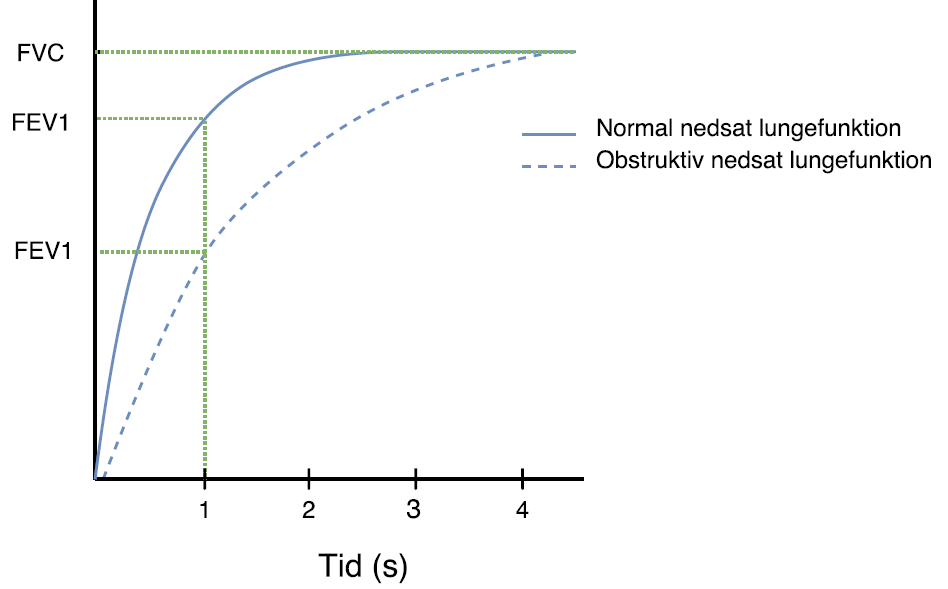
\includegraphics[width=0.8\textwidth]{figures/FEV}
\caption{Spirometrimålinger for patienter med normal og obstruktiv nedsat lungefunktion. Revideret\cite{Basisbogen2016}.}
\label{fig:FEV}
\end{figure} 

\noindent
Det fremgår af \autoref{fig:FEV}, at der ved obstruktivt og restriktiv nedsat lungefunktion er et fald i FEV1 samt FVC. Der udføres ligeledes en reversibilitetstest for at sikre, at patienter ikke lider af differentialdiagnosen astma. Disse patienter gives broncodilatorer, som hos astmapatienter vil forbedre spirometrimålingen, mens lungefunktionen for KOL-patienter forbliver uændret.\cite{Basisbogen2016, Sundhed2013} 
For at undersøge KOL og patienters komorbiditeter undersøges foruden lungefunktionsundersøgelser også BMI, røntgen af thorax, EKG-målinger og blodprøver \cite{Sundhed2013}. 
%Med tiden kan symptomerne på KOL forværres, og der skal mindre fysisk aktivitet til for at udløse åndenød. \cite{Basisbogen2016}
\subsubsection{Klassifikation af KOLs sværhedsgrad} \label{sec:klassifikation}
Sværhedsgraden af KOL vurderes på baggrund af patienters symptomer, egne erfaringer og livskvalitet. Denne vurderes ud fra Medical Research Council åndenødsskala (MRC) eller Chronic obstructive pulmonary disease Assessment Test (CAT). Patienter kan efterfølgende inddeles i klassifikationer med udgangspunkt i MRC, CAT eller ved spirometrimålinger.\cite{Basisbogen2016}

 
MRC-skalaen er en skala fra $1$ til $5$, hvor patienter vurderer mængden af aktivitet, som de kan udføre i forhold til åndenød. Skalaen fremgår af \autoref{tab:MRC}, hvor $1$ svarer til, at patienter først oplever åndenød ved meget anstrengelse, og $5$ svarer til, at patienter oplever åndenød ved meget lav fysisk aktivitet.\cite{Basisbogen2016}

\begin{table} [H]
\centering
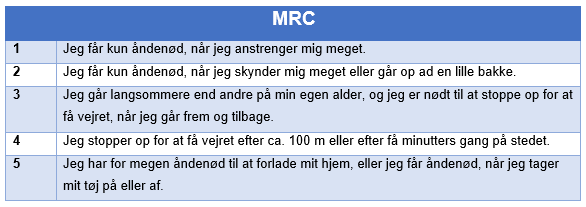
\includegraphics[width=0.9\textwidth]{figures/MRC}
\caption{MRC er en skala fra $1$ til $5$. Patienter, der oplever åndenød ved meget anstrengelse vurderes til $1$, mens patienter, der oplever åndenød ved lav aktivitet vurderes til $5$ på MRC-skalaen. Revideret\cite{Basisbogen2016}.}
\label{tab:MRC}
\end{table} 

\noindent
En anden metode til at vurdere symptomerne ved KOL er ved hjælp af CAT-spørgeskema. Her vurderes otte udsagn fra en skala fra $0$ til $5$, hvor ingen symptomer angives $0$. Ud fra de otte udsagn opnås en samlede score, jo højere den samlede score er, desto værre opleves patienters symptomer. Af \autoref{fig:CAT} ses CAT-spørgeskema til vurdering af symptomer.\cite{dsam2016,Basisbogen2016}

\begin{figure} [H]
\centering
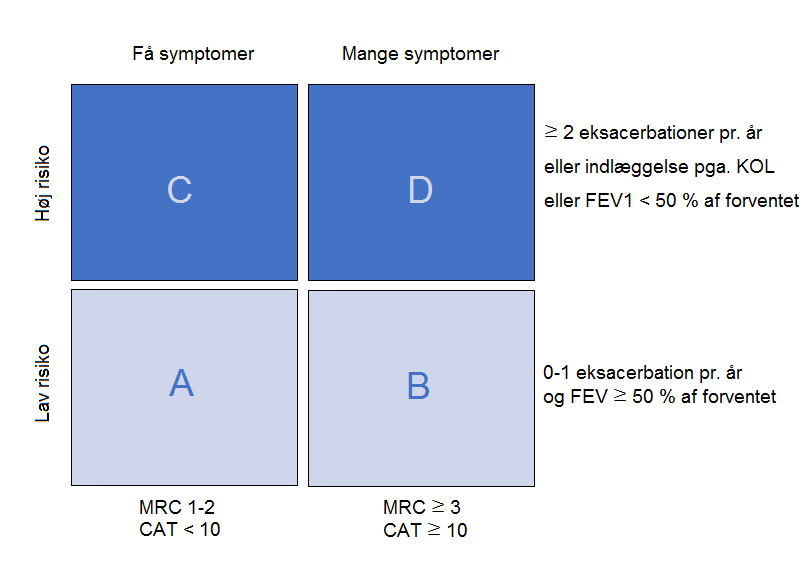
\includegraphics[width=0.5\textwidth]{figures/CAT}
\caption{CAT er et spørgeskema, hvor patienter vurderer graden af deres symptomer ud fra otte udsagn på en skala fra $0$ til $5$. Ingen symptomer svarer til $0$. Patienter opnår en samlede score, jo højere den samlede score er, desto værre opleves patienters symptomer. Revideret\cite{Basisbogen2016}.}
\label{fig:CAT}
\end{figure} 

\noindent
Ud fra MRC-skalaen eller CAT-spørgeskemaet samt lungefunktionstest og antallet af eksacerbationer det seneste år kan KOL-patienter kategoriseres. Patienterne kategoriseres i A, B, C eller D, hvor D er patienter i høj risiko og med mange symptomer. Kategoriseringen fremgår af \autoref{fig:KAT}.

\begin{figure} [H]
\centering
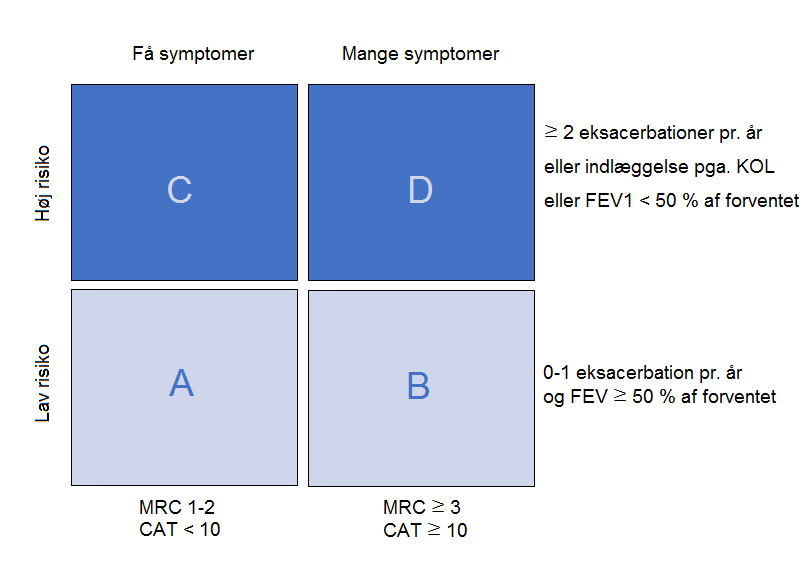
\includegraphics[width=0.8\textwidth]{figures/KAT}
\caption{KOL-patienter kategoriseres i fire kategorier herunder A, B, C og D. A og B inddeles i lav risiko, mens C og D er i høj risiko. Revideret\cite{Basisbogen2016}.}
\label{fig:KAT}
\end{figure} 
 
\noindent
Udover ABCD-kategoriseringen kan sværhedsgraden af KOL udelukkende bestemmes ud fra spirometrimålinger.  Sværhedsgraden er klassificeret ud fra retningslinjer opstillet af the Global Initiative for Chronic Obstructive Lung Disease (GOLD).\cite{dsam2016} Lungefunktionen vurderes på baggrund af FEV$1$ i \% af den forventede lungekapacitet, hvoraf det inddeles i fire stadier. Disse fremgår af \autoref{tab:GOLD}.

\begin{table} [H]
\centering
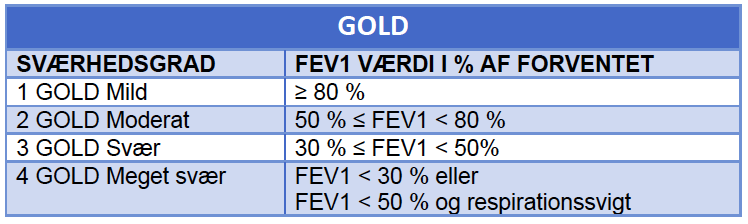
\includegraphics[width=0.8\textwidth]{figures/GOLD}
\caption{GOLD er inddelt efter sværhedsgraderne $1$ til $4$ herunder mild, moderat, svær og meget svær. Patienter, der har over $80~\%$ af forventet lungekapacitet klassificeres som $1$ GOLD mild, mens patienter med under $30~\%$ eller over $50~\%$ af forventet lungekapacitet samt respirationssvigt klassificeres som $4$ GOLD meget svær. Revideret\cite{Basisbogen2016}.}
\label{tab:GOLD}
\end{table} 

\subsection{Behandling} \label{sec:behandling}
Det er ikke muligt at helbrede patienter med KOL, da KOL er en kronisk lungesygdom. Dog er det muligt at forhindre udviklingen af KOL samt lindre symptomerne, hvilket kan opnås ved tobaksafvænning, fysisk aktivitet, kostvejledning og medicin.\cite{Basisbogen2016} 

KOL-patienter med sekretproblemer tilbydes continous positive airway pressure (CPAP) eller positive expiratory pressure (PEP-fløjte) og broncodilaterende inhalationsbehandling efter behov og ud fra graden KOL. Yderligere kan antiinflammatorisk behandling gives til patienter med hyppige eksacerbationer.\cite{Basisbogen2016}

Da den tabte lungefunktion ikke kan genvindes, rådes patienterne til ophøre tobaksrygning eller det der kan være årsagen til KOL f.eks. dårligt arbejdsmiljø, hurtigst muligt for således at bibeholde den nuværende lungefunktion \cite{Basisbogen2016}. Det fremgår af \autoref{fig:fletcher}, hvordan tobaksrygning kan påvirke lungefunktionen over tid. 

\begin{figure} [H]
\centering
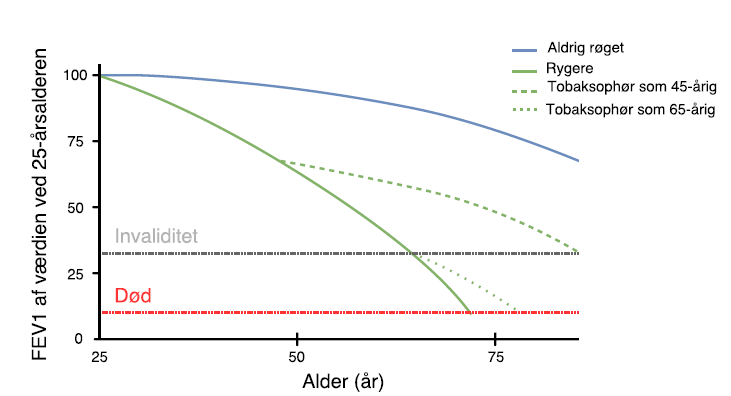
\includegraphics[width=1\textwidth]{figures/fletcher}
\caption{Fletcher-kurve, som viser faldet af FEV1 over tid for henholdsvis rygere, ikke-rygere og rygere med tobaksophør i $45$- og $65$-årsalderen. Revideret\cite{Basisbogen2016}.}
\label{fig:fletcher}
\end{figure} 

\noindent
Det ses af \autoref{fig:fletcher}, at tobaksrygning medvirker til et accelererende tab af FEV1, og dermed udsigt til kortere levetid. På trods af tobaksophør genoprettes FEV$1$ ikke, dog bremses det accelerende tab af FEV$1$ til det normale aftag.\cite{dsam2016}

\subsection{Prognose}
KOL-patienter med eksacerbationer har efter indlæggelse en dødelighed på næsten $10$~$\%$ i løbet af den første måned. Dødeligheden ligger på omkring $64$ per $100.000$ per år for mænd og $54$ per $100.000$ per år for kvinder.
Udviklingen, hvormed sygdommen progredierer for KOL-patienter er specielt afhængig af, hvorvidt patienter ophører eksponering til den udløsende faktor for eksempel tobaksophør. Det er derfor vigtigt at få en tidlig diagnosticering således, at patienter hurtigt kan få hjælp.\cite{dsam2016}
%Derudover har et studie vist, at KOL-patienter, der er i stadie $4$ i GOLD-klassificeringen, har lav funktionalitet og livskvalitet, som bliver værre med tiden og ved fremkomst af flere symptomer til sygdommen. \cite{Habraken2011}


\section{Rehabilitering}
Da KOL er kronisk lungesygdom, hvorved den tabte lungefunktion ikke kan genoprettes, tilbydes KOL-patienter rehabilitering med henblik på at mindske deres symptomer. 

I Danmark henvises KOL-patienter til rehabilitering fra praktiserende læge eller hospital. Rehabilitering forløber typisk over $8$ ugers periode på et sundhedscenter eller på et hospital. KOL-patienter møder til træning $1$-$2$ gange om ugen, de resterende dage vil patienten kunne udføre de fremviste øvelser hjemme. \cite{McCarthy2015}[lunge.dk/rehabilitering] 

Individuel rehabilitering anses som værende fundamental for KOL-patienter, hvor forløbet tilpasses i forhold til patienternes behov med henblik på at opnå det bedste udbytte af rehabiliteringen \cite{McCarthy2015,Habraken2011}[sundkol2015]. Ligeledes vurderes rehabiliteringen på baggrund af graden af KOL, da KOL fremkommer i flere grader samt med varierende progression \cite{McCarthy2015}. 

Rehabiliteringen kan give patienter bedre mulighed for deltagelse i hverdagen, såfremt patienters tilstand tillader det. \cite{McCarthy2015,Habraken2011} [sundkol2015] Opfølgninger kan foretages efter rehabiliteringsforløb er afsluttet, for at undersøge om patienter opretholder de gavnlige effekter. [lunge.dk/rehabilitering]


\subsection{Rehabiliteringsforløbet}
Rehabiliteringsforløbet fokuserer på tobaksafvænning, fysisk træning, kendskab til sygdommen samt ernæringsvejledning. \cite{McCarthy2015,Habraken2011} [sundkol2015] 

Tobaksafvænning er, som beskrevet i \autoref{sec:behandling}, et relevant element i forhold til at begrænse udviklingen af sygdommen og bevare mest mulig lungefunktion. Den fysiske træning, der udføres under rehabiliteringen, medvirker til, at patienter kan opnå et bedre udbytte af den resterende lungefunktion, samt opnå et bedre fysisk funktionsniveau [sundkol2015]. 
Træningen vil ligeledes modvirke eventuelle følger ved KOL, da fysisk træning øger muskelfunktionen samt udsætter træthed, hvilket medfører forøget aktivitetstolerance \cite{McCarthy2015}. Dog kan den fysiske træning resultere i åndenød hos KOL-patienter, der kan forstærkes, hvis patienter påvirkes af angst som følge af åndenød. Dette kan betyde, at KOL-patienter afholder sig fra fysisk træning på grund af frygten for angst. \cite{McCarthy2015} [sundKOL2015]. 

Et led i rehabiliteringen er ligeledes, at patienter opnår viden indenfor sygdomshåndtering, der omhandler kendskab til og forebyggelse af sygdommen, livsstilsændringer samt håndtering af eksacerbationer\cite{McCarthy2015} [sundKOL2015]. Her fokuseres blandt andet på de gavnlige effekter ved tobakophør og regelmæssig fysisk aktivitet, samt hvornår og hvordan eventuel medicin skal indtages. Patienten vil yderligere blive introduceret til energibesparende strategier og vejrtrækningsøvelser \cite{McCarthy2015} [sundkol2015].   


\section{Problemformulering}
\textit{Hvordan udvikles en app til at vejlede og motivere KOL-patienter til hjemmetræning i forlængelse af rehabiliteringsforløb med henblik på at mindske symptomer forbundet med KOL? }

%-----------------------Problemanalyse---------------------------
\chapter{Metode}
***    Mangler indledning (evt. hvorfor vi bruger OOP)   *****

\section{Objektorienteret programmering}
Objektorienteret programmering er et programmeringsparadigme, som anvendes til at analysere, designe, implementere samt udvikle app's. Hyppige termer inden for objektorienteret programmering er blandt andet objekter, klasser, indkapsling, nedarvning og polymorfi.\cite{Stefanov2013,Brahma2015}

I objektorienteret programmering opdeles programmeringskoden i klasser, hvor hver klasse fungerer som en opskrift for et objekt. Hvert objekt er en instans af en bestemt klasse, hvor en klasse kan være bygget op omkring en eller flere instanser. De forskellige objekter repræsenterer hver sin del af app'en og indeholder data og logik. Derudover har objekterne mulighed for at kommunikere mellem hinanden. Objekter er karakteriseret ud fra deres egenskaber, og deres funktioner er beskrevet ved metoder.\cite{Stefanov2013,Brahma2015} Eksempler på egenskaber og metoder fremgår af \autoref{tab:objekt}. 

\begin{table}[H]
\centering
\begin{tabular}{|l|l|}
\hline
\textbf{Egenskaber} & \textbf{Metoder} \\ \hline
\begin{tabular}[c]{@{}l@{}}Navn \\ Køn\\ Alder\\ Højde \\ Vægt\end{tabular} & \begin{tabular}[c]{@{}l@{}}Gå\\ Løbe\\ Hoppe\\ Sove\\ Tale\end{tabular} \\ \hline
\end{tabular}
\caption{Objekter karakteriseres ud fra deres egenskaber som for eksempel navn, mens metoder beskriver deres funktion som for eksempel sove.}
\label{tab:objekt}
\end{table}

\noindent
Objektorienteret programmering består af tre grundprincipper, herunder indkapsling, nedarvning og polymorfi. Indkapsling er en illustration af, at objekter både indeholder egenskaber og metoder. Egenskaber opbevarer data, mens metoder anvendes til at behandle data. Indkapsling kan både have synlige og skjulte informationer. Synlig information udgør  ofte grænsefladen, såsom knapper og display, mens skjult information kan være implementeringen af grænsefladen. Dette gør sig også gældende for objekter, hvilket defineres som public eller private. Ved public har alle objekter adgang til metoderne, mens private kun er metoder med samme objekt, der kan tilgå denne. Nedarvning betyder, at et objekt kan arve data og funktioner fra et andet objekt. Dette muliggør, at objektet kan udvides med ekstra data og funktioner. Polymorfi giver mulighed for, at to klasser kan have samme grænseflade. Denne er defineret ved nedarvningen.\cite{Stefanov2013}


%%-----------------------System udvikling-------------------------
\chapter{Systemudvikling}

%%-----------------------Teori-------------------------




%%-----------------------Implementering-------------------------


%%-----------------------Test-------------------------%%


%\iffalse
\begingroup
\raggedright

\bibliographystyle{unsrtnat}
\bibliography{kilder123}
%\urlstyle{same}
%
%
%\printbibliography
%\cleardoublepage

\endgroup

%-----------------------Bilag-------------------------
\appendix

%\fi
\end{document}
